\documentclass[12pt]{article}

\usepackage{graphicx}
\usepackage{epstopdf}


\usepackage[spanish]{babel} % silabea palabras castellanas <- Puedo poner comentarios para explicar de que va este comando en la misma línea
\selectlanguage{spanish} 

%Encoding
\usepackage[utf8]{inputenc} % Acepta caracteres en castellano
\usepackage[T1]{fontenc} % Encoding de salida al pdf

%Triunfó el mal
\usepackage[normalem]{ulem}
\useunder{\uline}{\ul}{}
\providecommand{\e}[1]{\ensuremath{\times 10^{#1}}}
\usepackage{quotmark} %Uso consistente con la RAE de comillas
\usepackage{listings} % Comandos de la terminal

\usepackage{textcomp}
\usepackage{gensymb}


%Hipertexto
\usepackage[colorlinks=true,urlcolor=blue,linkcolor=blue]{hyperref} % navega por el doc: hipertexto y links

%Aquello de las urls
\usepackage{url} 

%simbolos matemáticos
\usepackage{amsmath}
\usepackage{amsfonts}
\usepackage{amssymb}
\usepackage{physics} %Best pack

% permite insertar gráficos, imágenes y figuras, en pdf o en eps
\usepackage{graphicx}
\usepackage{epstopdf}
\usepackage{multirow}
\usepackage{float}
\usepackage[export]{adjustbox}
% geometría del documento, encabezados y pies de páginas, márgenes
\usepackage{geometry}
\usepackage{comment}

%\usepackage[english]{babel}
%\usepackage[latin5]{inputenc}
% \usepackage{hyperref}
%\newdate{date}{10}{05}{2013}
%\date{\displaydate{date}}
\begin{document}




\title{Cúmulos Abiertos \\ Taller 4 fotometría de apertura con PHOT}

\author{
\textbf{Javier Alejandro Acevedo Barroso\thanks{e-mail: \texttt{ja.acevedo12@uniandes.edu.co}}}\\
\textit{Universidad de los Andes, Bogotá, Colombia}\\
 }% Hasta aquí llega el bloque "author" (son dos autores por informe, orden alfabético)

\date{\today}
%\date{Versión $\alpha \beta$ fecha del documento}
\maketitle %Genera el título del documento


\normalsize
\newpage



\section{Fotometría de apertura}
EL objetivo del ejercicio es realizar el procesamiento de fotometría de apertura a las imágenes ciencia del ejecicio \tqt{Photom} de IRAF. En esta ocasión se utilizará la tarea PHOT en vez de QPHOT.
Las imágenes a usar ya tuvieron la respectiva corrección de BIAS, OVERSCAN y FLAT. Adicionalmente, en el desarrollo del ejercicio anterior se les agregó la masa de aire a su \tqt{header}, de modo que se puede proceder a la fotometría.\\

El primer paso será encontrar las estrellas a usar. Anteriormente, esto se hacía manualmente con la tarea IMEXAMINE. 
Ahora, se usará la tarea DAOFIND para automatizar la búsqueda de estrellas en las imágenes. 
La tarea DAOFIND pertenece al paquete DIGIPHOT y APPHOT. 
Esta tarea requiere de la desviación estándar del {fondo} de la imagen y del FWHM del perfil radial, ambos datos se pueden obtener con la tarea IMEXAMINE.
Del ejercicio anterior sabemos que las estrellas tienen un FWHM de 2.65 a 3.2, se tomará 3 como FWHM. Para la desviación estándar del fondo se tomó 9.2.
Por último, durante la ejecución de DAOFIND se debe especificar el valor de la desviación estandar mínimo de una región para ser considerada un objeto.    	\\

Tras correr DAOFIND, se puede utilizar la tarea TVMARK para visualizar las estrellas encontradas.
Para un DAOFIND con FWHM de 3 pixeles y un \tqt{sigma} de 9.2 se obtuvieron 81 estrellas, la visualización de TVMARK se puede observar en la figura \ref{im1}.\\

Tras ubicar las estrellas, se procede a hacer la fotometría con PHOT.
Esta requiere seleccionar un algoritmo de centrado (que permite utilizar el mismo archivo de coordenadas para todas las imágenes pues garantiza que las coordenadas siempre tomarán el centro de una estrella), el tamaño en pixeles de la caja de centrado para el algoritmo de centrado (en este caso se tomará 5 pixeles), la variable estadística a tomar para el valor del anillo del cielo (moda, media, mediana o centroide. En este caso se eligió la mediana), el radio interior del anillo del cielo (15 pixeles), el radio del anillo de cielo (10 pixeles) y el radio de la apertura (15 pixeles). 
Tras ejecutar PHOT, se obtuvo datos de fotometría para 73 objetos. Para los 8 restantes, IRAF fue incapaz de dar una magnitud y solo responde \tqt{INDEF}.


\begin{figure}[H]
   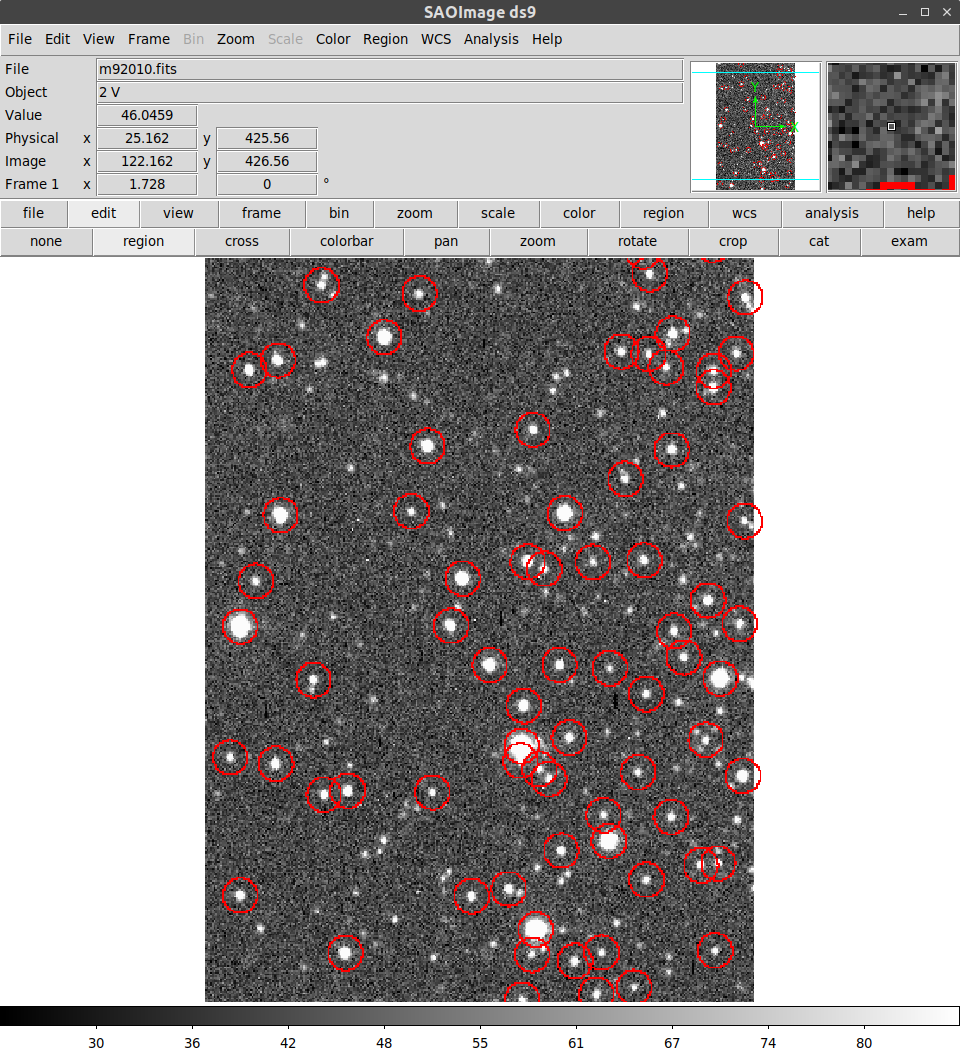
\includegraphics[scale=0.4]{im01.png}
  \caption{Estrellas seleccionadas para la fotometría de apertura en la imagen m92010.}
  \label{im1}
\end{figure}


En las tablas a continuación se reportan los resultados. Para cada imagen se tiene una tabla con: título de la imagen, coordenadas del objeto, magnitud e incertidumbre de la magnitud.









%\bibliography{bibTes}{}
%\bibliographystyle{unsrt}


\end{document}




\begin{figure}[H]
  \centering
   \includegraphics[scale=•]{•}= 0.65]{im03.png}
  \caption{Cargando las imágenes a diferentes frames de DS9 desde la sesión de IRAF. }
  \label{im03}
\end{figure}





\section{Cronograma}

\begin{table}[htb]
	\begin{tabular}{|c|cccccccccccccccc| }
	\hline
	Tareas $\backslash$ Semanas & 1 & 2 & 3 & 4 & 5 & 6 & 7 & 8 & 9 & 10 & 11 & 12 & 13 & 14 & 15 & 16  \\
	\hline
	1 & X & X & X  &   &   &   &   &  &  &   &   &   &   &   &   &   \\
	2 &   &  & X & X & X &  &  &   &   &  &  &  &   &  &  &   \\
	3 &   &   &   &  & X  & X  & X  & X &   &   &   &  &   &   &  &   \\
	4 &  &  &  &  &  &  &  & X & X & X & X &   &   &   &   &   \\
    5 &  &  &  &  &  &  & X & X &  &  &  &   &   &   &   &   \\
	6 &   &   &   &   &  &   &  X & X  &  &   &  X & X &  X & X  & X &   \\
	\hline
	\end{tabular}
\end{table}
\vspace{1mm}
 %CCDRED se encarga de la corrección en sí, sus parámetros son: el tipo de dato de los pixeles (real, short, etc), el nombre del backup (en caso de querer un backup), el archivo de traducción del instrumento (que para una CCD estandar ya viene incluido en IRAF